\section{Global Navigation Satellite Systems (GNSS)}

\begin{frame}{Trilateration in GNSS networks}

    System of equations involved in trilateration \textbf{($\delta t$ is the receiver clock delay)}:

    \begin{equation*}
        \Delta d_i = c \cdot (\Delta t_i + \delta t) = \sqrt{(x_r - x_i)^2 + (y_r - y_i)^2 + (z_r - z_i)^2}, \quad i = 1, 2, 3, 4
    \end{equation*}

    \begin{columns}[c, onlytextwidth]

        \begin{column}{0.6\textwidth}

            \begin{equation*}
                \underbrace{x_r, y_r, z_r, \delta t}_\text{4 Unknowns requires 4 satellites}
            \end{equation*}

            \vspace{10pt}

            \textbf{Final position strongly depends on $\delta t$.}

        \end{column}

        \begin{column}{0.4\textwidth}

            \begin{figure}[H]
                \centering
                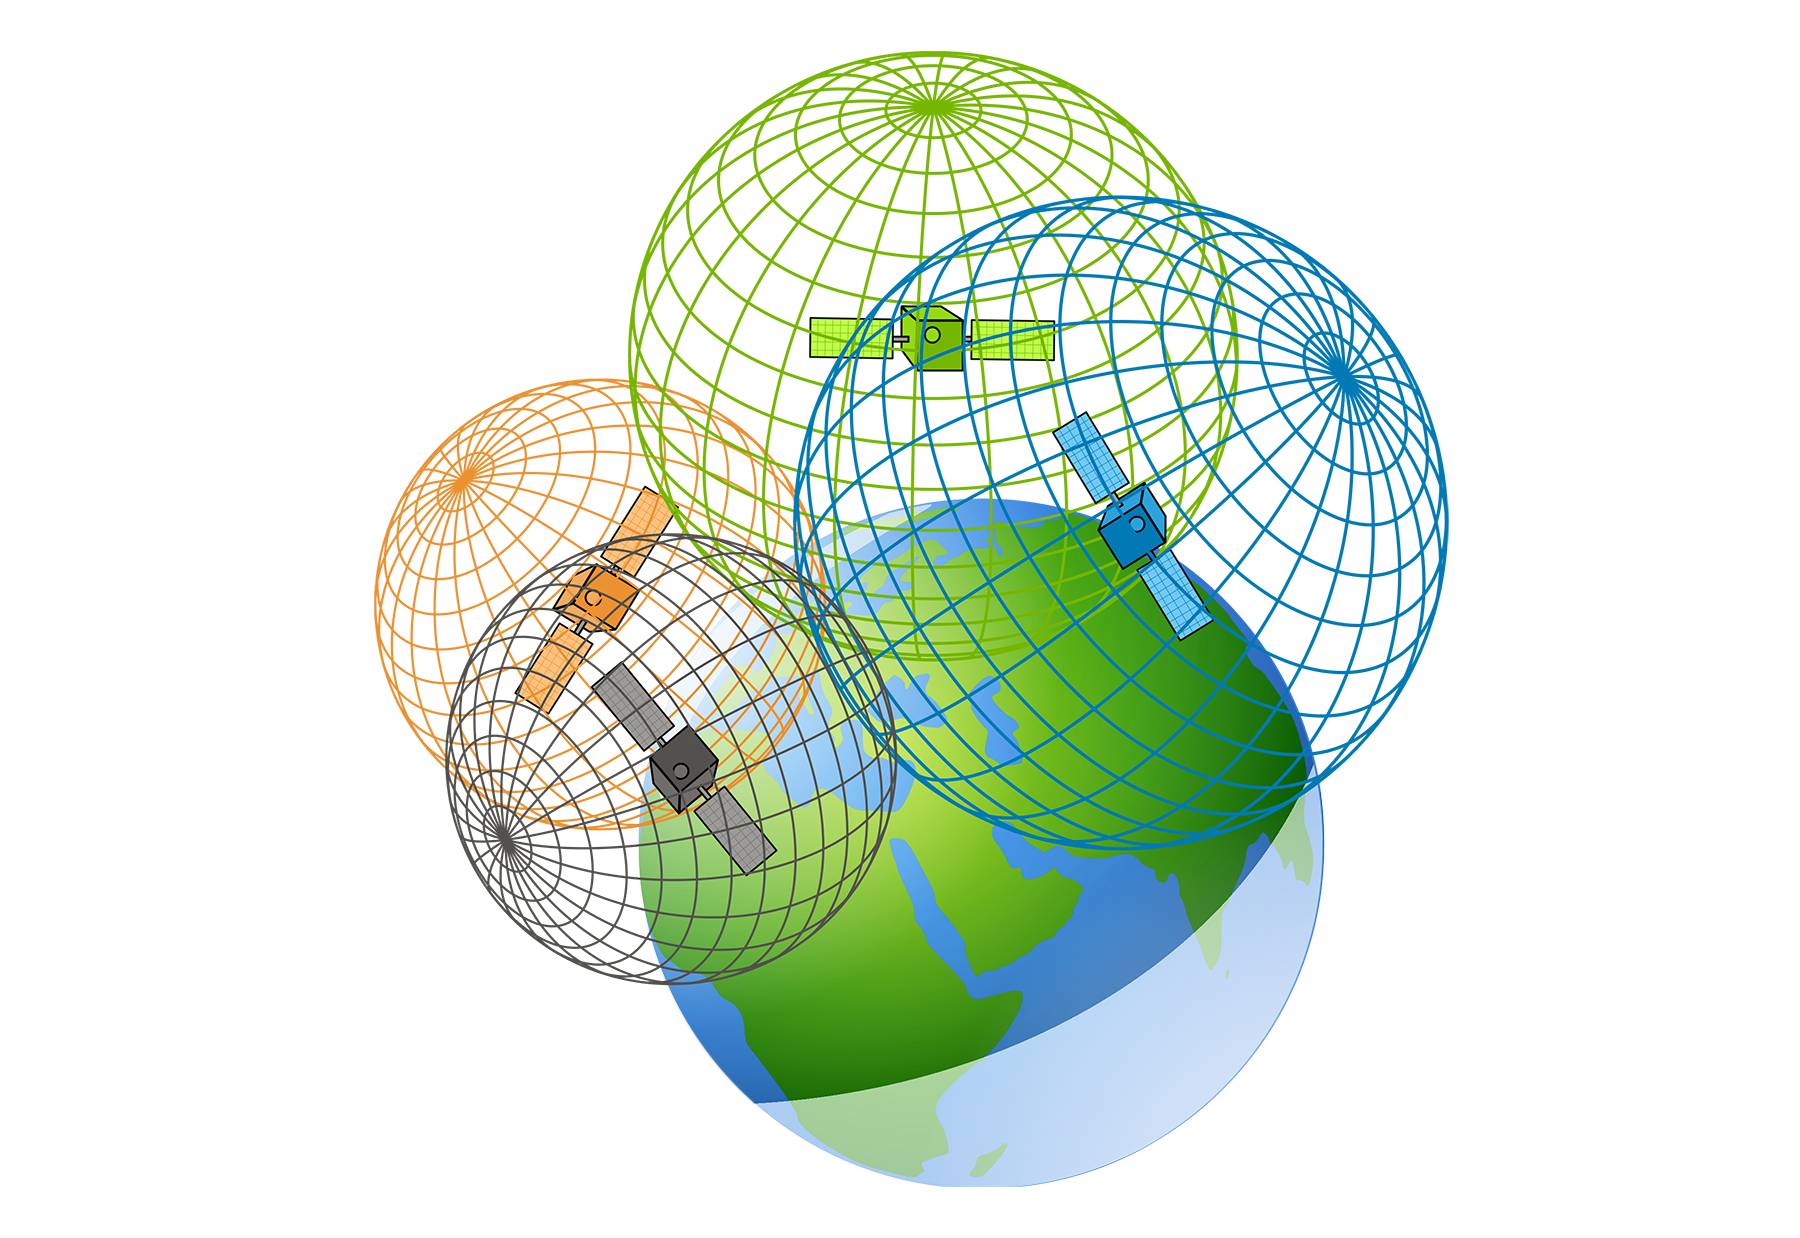
\includegraphics[width=\textwidth]{img/GPS-Trilateration.png}
                % \caption{GPS trilateration}
            \end{figure}

        \end{column}

    \end{columns}

    \footnotetext{In the equation above, $c$ is the speed of light which is approximately $3 \times 10^8$ m/s.}

\end{frame}



% \begin{frame}{Role of CSAC}

%     Better holdover capabilities $\rightarrow$ eliminate the need for the 4\textsuperscript{th} satellite after the first clock calibration.

%     More accurate timing $\rightarrow$ more precise trilateration and indeed a more accurate position.

%     \vspace{10pt}

%     \begin{columns}[c, onlytextwidth]

%         \begin{column}{0.5\textwidth}

%             % TODO: change image, take the one from Travagning p.68
%             \begin{figure}
%                 \centering
%                 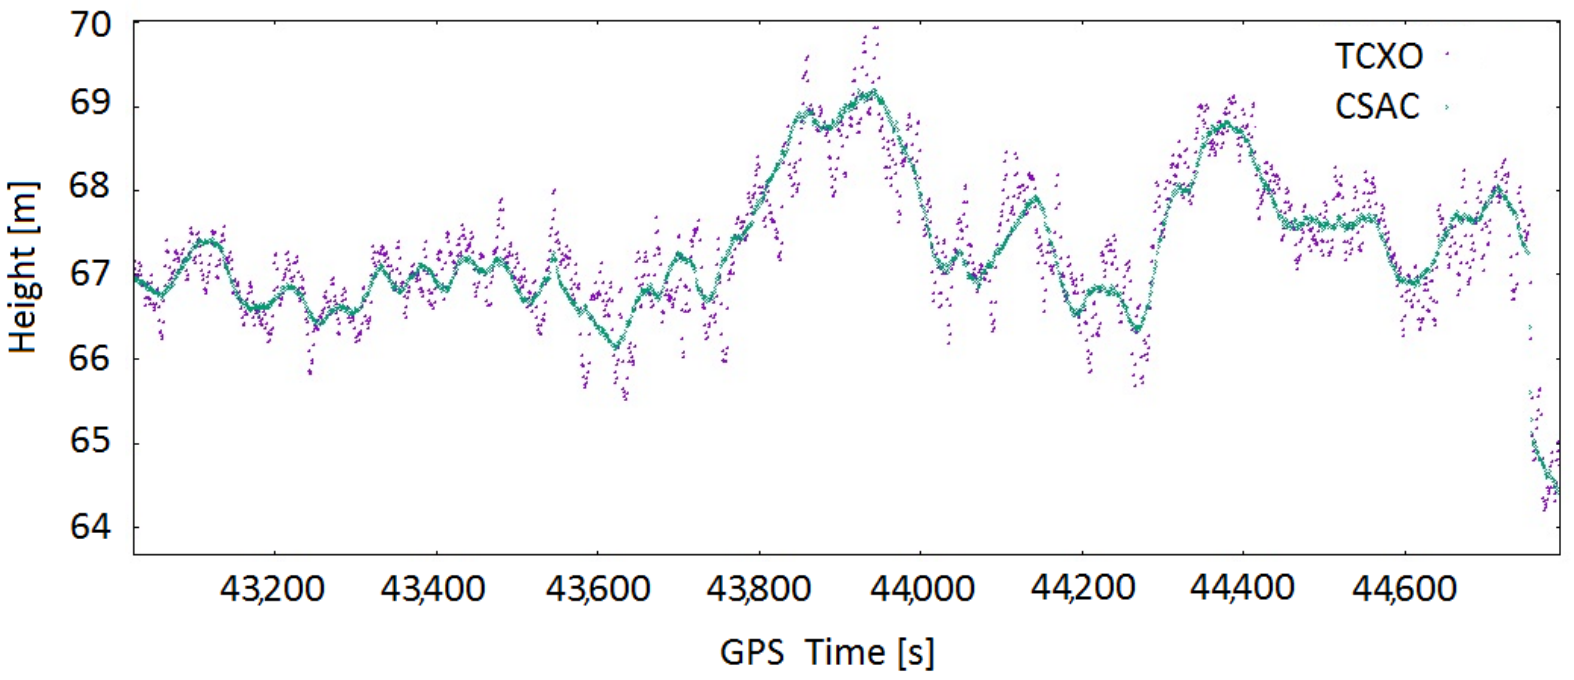
\includegraphics[width=\textwidth]{img/GNSS-height.png}
%                 \caption{
%                     \textcolor[HTML]{663B7A}{TCXO},
%                     \textcolor[HTML]{64857B}{CSAC}
%                 }
%             \end{figure}

%         \end{column}

%         \hfill

%         \begin{column}{0.45\textwidth}

%             \begin{table}
%                 \centering
%                 \resizebox{\textwidth}{!}{
%                     \begin{tabular}{l|cc}
%                         ~    & \textbf{Static} & \textbf{Dynamic} \\
%                         ~    & (cm)            & (cm)             \\
%                         \hline
%                         TCXO & 50.0            & 55.0             \\
%                         CSAC & 25.5            & 24.3             \\
%                         \hline
%                     \end{tabular}
%                 }
%                 \caption{Height error standard deviation in static and dynamic conditions.}
%             \end{table}

%         \end{column}

%     \end{columns}

% \end{frame}



\begin{frame}{Role of CSAC}

    \begin{columns}[c, onlytextwidth]

        \begin{column}{0.55\textwidth}

            Better holdover capabilities $\rightarrow$ eliminate the need for the 4\textsuperscript{th} satellite after the first clock calibration.

            \vspace{10pt}

            More accurate timing $\rightarrow$ more precise trilateration and indeed a more accurate position.

        \end{column}

        \hfill

        \begin{column}{0.40\textwidth}

            \begin{figure}
                \centering
                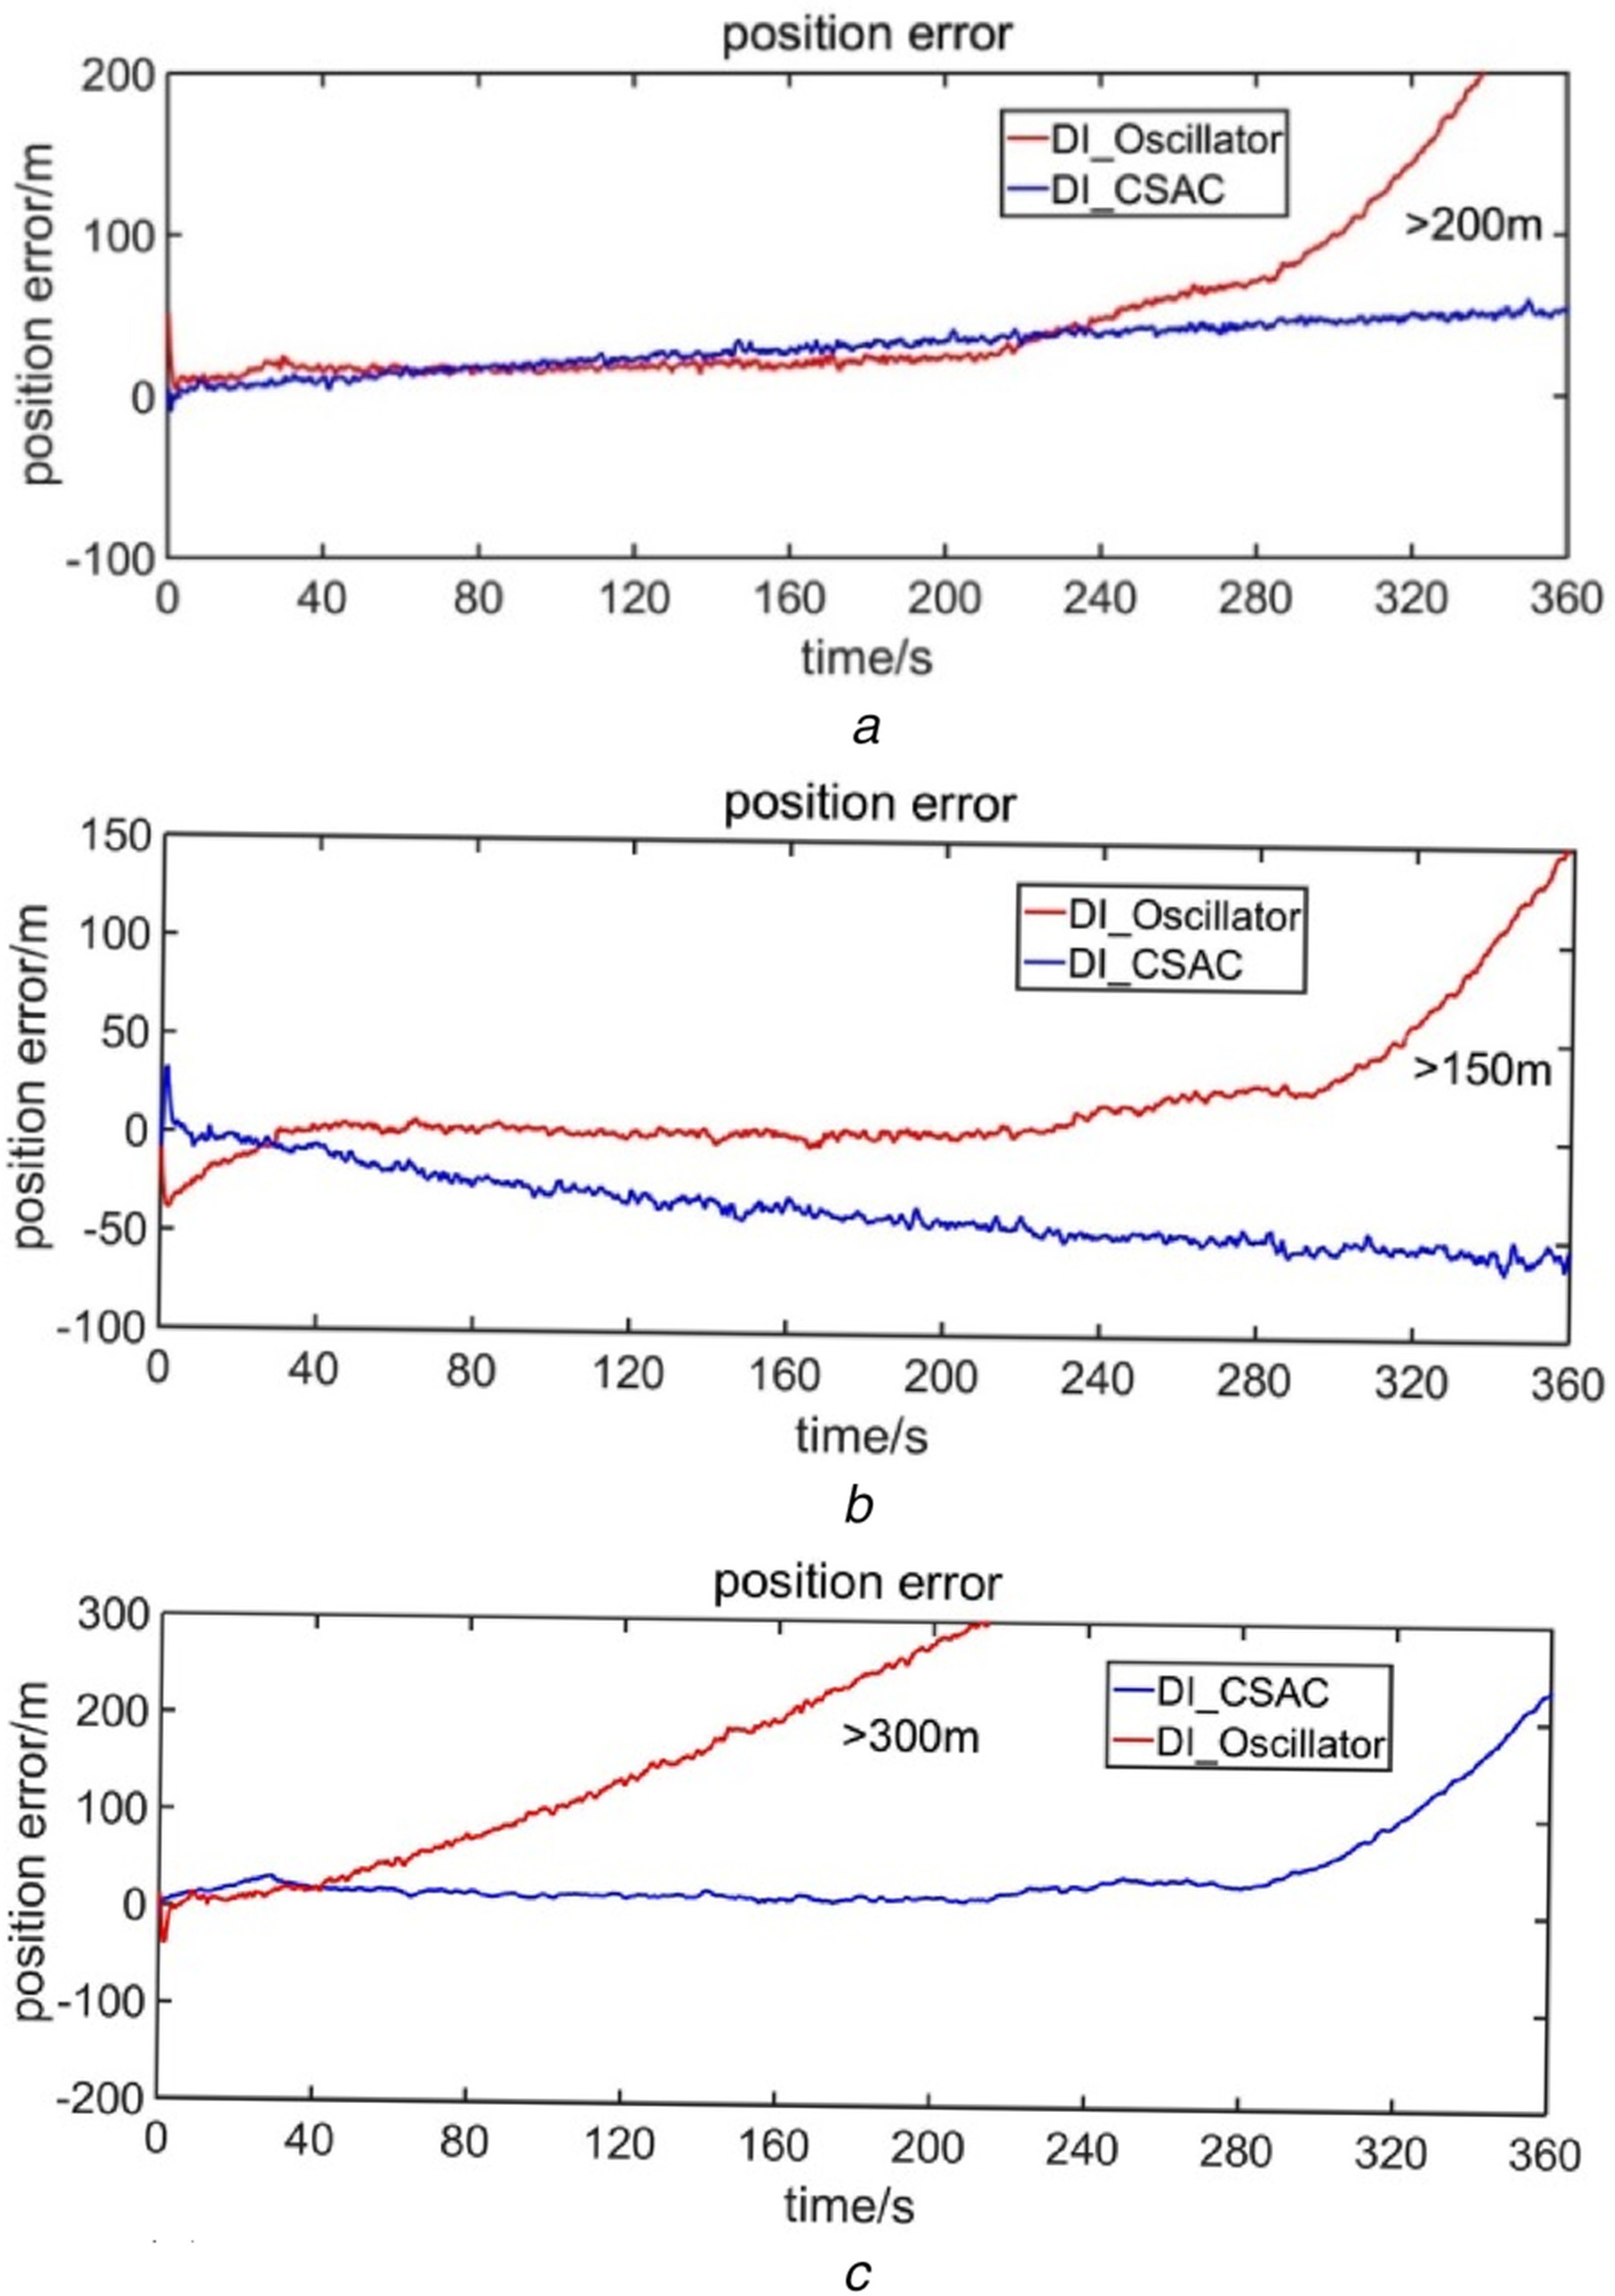
\includegraphics[width=\textwidth]{img/GNSS-errors.jpg}
                \caption{
                    \textcolor[HTML]{3E4091}{TCXO},
                    \textcolor[HTML]{B04A47}{CSAC}
                }
            \end{figure}

        \end{column}

    \end{columns}

\end{frame}

